\begin{frame}{Motivación 1/2}

    \begin{figure}[ht]
        \begin{center}
            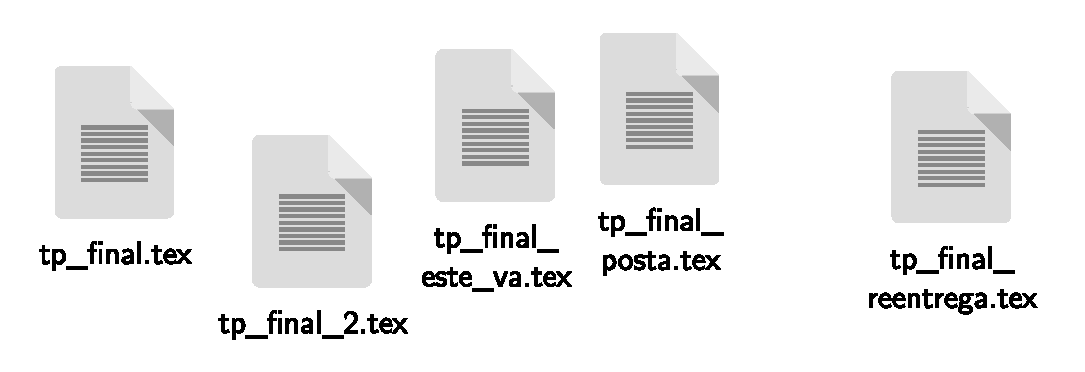
\includegraphics[height=1.5in]{images/caos.pdf}
        \end{center}
    \end{figure}

    \pause
    \begin{figure}[ht]
        \begin{center}
            
\includegraphics[height=1.5in]{images/horror.png}
        \end{center}
    \end{figure}

\end{frame}

\begin{frame}{Motivación 2/2}

    \begin{block}{Trabajando en grupo}
        \begin{itemize}
            \item Enviar cambios por mail, o
            \pause
            \item Sincronizar cambios por Dropbox, o
            \pause
            \item Sincronizar cambios por Google Docs.
        \end{itemize}
    \end{block}

    \pause
    \begin{figure}[h]
        \begin{center}
            
\includegraphics[height=1.5in]{images/horror.png}
        \end{center}
    \end{figure}

\end{frame}

\begin{frame}{¿Qué es un Sistema de Control de Versiones?}

	\begin{block}{}
		Los \textbf{Sistemas de Control de Versiones} son programas que permiten \textbf{manejar los cambios} en el código fuente de un proyecto a lo largo del tiempo.

		Llevan un \textbf{seguimiento} de las modificaciones que hacemos, y en caso de que nos equivoquemos, es posible volver atrás y comparar el código actual con versiones anteriores para ayudar a arreglar el error.

		También permiten que distintas personas modifiquen el código a la vez y \textbf{compartan los cambios}, tratando de prevenir conflictos, y en caso de que los hubiera, ayudando a identificarlos y resolverlos.

	\end{block}

    \pause
    \begin{resumen}{Es decir, permiten...}
        \begin{itemize}
            \item Arreglar \textit{accidentes} y volver a versiones anteriores del código.
            \item Compartir código con otras personas.
        \end{itemize}
	\end{resumen}

\end{frame}

\begin{frame}{¿Qué es Git?}

	\begin{block}{}
		Git es un Sistema de Control de Versiones \textbf{distribuido y de código abierto}.
        Además fue diseñado con énfasis en la \textbf{performance} (para manejar proyectos muy grandes), \textbf{seguridad} y \textbf{flexibilidad}.
        Provee un amplio conjunto de comandos que permiten realizar operaciones de alto y bajo nivel.
	\end{block}

    \begin{figure}[ht]
        \begin{center}
            
\includegraphics[height=1.5in]{images/logo-git.pdf}
        \end{center}
    \end{figure}
\end{frame}

\begin{frame}{All night ¿Git?}

    \begin{figure}[ht]
        \begin{center}
            
\includegraphics[height=1.5in]{images/homero-git.jpg}
        \end{center}
        \caption{Referencia: \url{https://youtu.be/Fi1aq0-H-jw}}
    \end{figure}
\end{frame}

\begin{frame}[fragile]{Configuraciones iniciales}

    \begin{block}{Tu identidad}
        Es importante establecer nuestro \textbf{nombre y email}, ya que estos van a ir asociados con los cambios que hagamos:

        \vspace{0.5em}

        \texttt{git config --global user.name "Guybrush Threepwood"}

        \texttt{git config --global user.email guybrush@example.com}
    \end{block}

\end{frame}

\begin{frame}[fragile]{Configuraciones iniciales}

	\begin{block}{Clave SSH}
		Para poder trabajar cómodamente con repositorios Git que estén en Internet (GitHub, Bitbucket, GitLab, etc.), podemos configurar una \textbf{clave SSH} que nos identifique con el servidor que estemos usando.
	\end{block}

  \pause
  \begin{block}{Creando una clave nueva}
		Abrimos la terminal y ejecutamos \code{ssh-keygen}. Le damos \textit{Enter} a todo.
	\end{block}

  \pause
  \begin{block}{Subiendo la clave a GitLab}
		\begin{itemize}
		  \item En la terminal, ejecutamos \code{cd ~/.ssh}, y luego \code{cat id\_rsa.pub}. Copiamos todo lo que aparezca.
      \item Abrimos GitLab, vamos a Profile Settings, SSH Keys.
      \item Pegamos lo que habíamos copiado en el campo \textit{Key}, y le ponemos un \textit{Title}, como por ejemplo \textit{Notebook del abuelo}.
      \item Le damos al boton \textit{Add key}.
		\end{itemize}
	\end{block}

\end{frame}

\begin{frame}[t]{Obteniendo un repositorio Git}

    \begin{comando}
        git clone
    \end{comando}

    \pause
	\begin{block}{}
        Para obtener una copia local de un repositorio existente en algún servidor,
        utilizamos el comando \texttt{git clone [URL]} (sin los corchetes).
    \end{block}

    \pause
    \vspace{1em}
    \begin{ejercicio}{Ejercicio}
        \textit{Clonar} el repositorio que tiene URL: \textbf{git@gitlab.com:talleres-comcom/taller-git-ejercicio.git}
    \end{ejercicio}
\end{frame}

\begin{frame}[t]{Preparando cambios}
    \begin{comando}
        git add
    \end{comando}

    \pause
    \begin{block}{}
        Una vez que tenemos cambios hechos, tenemos que marcarlos como preparados antes de confirmarlos. En la jerga de Git, decimos que pasamos los cambios a \textit{staged}.
        \begin{enumerate}
            \item Creamos/modificamos el archivo en cuestión.
            \item Ejecutamos \texttt{git add [nombre del archivo]}.
        \end{enumerate}
    \end{block}

    \pause
    \vspace{1em}
    \begin{ejercicio}{Ejercicio}
        Adentro del repositorio que \textit{clonaron} recién, crear un archivo y
        marcarlo como \textit{staged} usando el comando \texttt{git add}.
    \end{ejercicio}
\end{frame}

\begin{frame}[t]{Confirmando cambios}
    \begin{comando}
        git commit
    \end{comando}

    \pause
    \begin{block}{}
        Una vez que tenemos ciertos cambios en \textit{staged}, podemos confirmarlos
        ejecutando \texttt{git commit -m [mensaje]}.

        \vspace{0.5em}

        Donde \texttt{[mensaje]} es una breve descripción de los cambios que acabamos de confirmar.
    \end{block}

    \pause
    \vspace{1em}
    \begin{ejercicio}{Ejercicio}
        Confirmar los cambios que pasaron a \textit{staged} en la diapo anterior.
    \end{ejercicio}
\end{frame}

\begin{frame}[t]{¡No seas vago con los mensajes!}

    \begin{figure}[ht]
        \begin{center}
            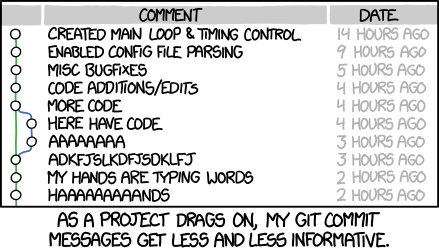
\includegraphics[height=2in]{images/xkcd-git-commit.png}
        \end{center}
        \caption{Fuente: \url{https://xkcd.com/1296/}}
    \end{figure}

\end{frame}

\begin{frame}[fragile, t]{¿Está preparado, confirmado o ninguna de las dos?}
    \begin{comando}
        git status
    \end{comando}

    \begin{block}{¡No es lo mismo!}
        Las modificaciones que hacemos pueden estar en \textbf{4 estados} distintos:
        \begin{itemize}
            \pause
            \only<-2>{\item \textbf{Sin seguimiento (untracked)}: archivos que nunca fueron agregados al repositorio, por ejemplo archivos nuevos.}
            \only<3-3>{\item \textbf{Modificado (modified)}: las modificaciones todavía no están marcadas como \textit{staged}.}
            \only<4-4>{\item \textbf{Preparado (staged)}: las modificaciones están en \textit{staged} e
                irán en la próxima \textit{confirmación de cambios} (\textit{commit}).}
            \only<5-5>{\item \textbf{Confirmado (committed)}: las modificaciones están guardadas con un \textit{mensaje} que explica los cambios realizados.}
        \end{itemize}
    \end{block}

    \only<2> {
        \begin{block}{Output de ejemplo}
            \gitstatusuntracked
        \end{block}
    }
    \only<3> {
        \begin{block}{Output de ejemplo}
            \gitstatusmodified
        \end{block}
    }
    \only<4> {
        \begin{block}{Output de ejemplo}
            \gitstatusready
        \end{block}
    }
    \only<5> {
        \begin{block}{Output de ejemplo}
            \gitstatusclean
        \end{block}
    }
\end{frame}

\begin{frame}{Colaborando con otras personas}

    Los repositorios remotos son \textit{copias} de nuestro proyecto a las cuales accedemos a través
    de Internet. Puede haber varios, cada uno de los cuales
    puede ser de solo lectura o de lectura/escritura, según los permisos que tengamos.

    \begin{figure}[ht]
        \begin{center}
            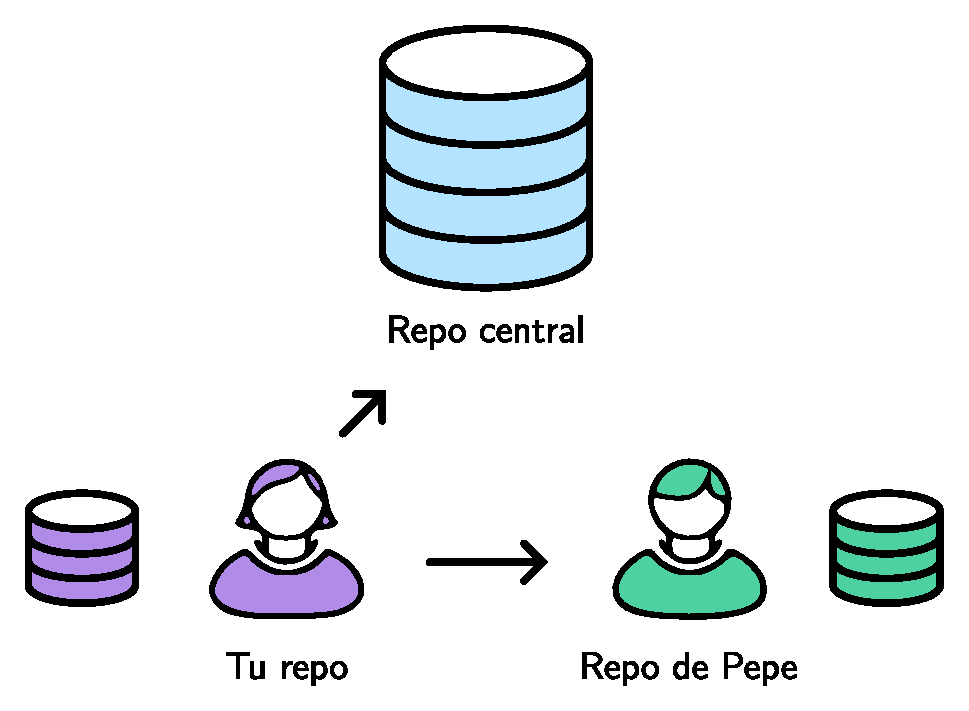
\includegraphics[height=1.5in]{images/repo-remoto.pdf}
        \end{center}
    \end{figure}

    Colaborar con otros implica gestionar estos repositorios remotos, y mandar (\textbf{push}) y recibir (\textbf{pull})
    datos de ellos cuando necesites compartir cambios.

\end{frame}

\begin{frame}[t]{Enviando cambios}
    \begin{comando}
        git push
    \end{comando}

    \pause
    \begin{block}{}
        Para enviar los cambios \textbf{desde nuestro repositorio local a algún
        repositorio remoto}, ejecutamos: \texttt{git push [remoto] [branch]}.

        \vspace{0.5em}

        Por ahora, hasta la siguiente clase, vamos a usarlo como:\\ \texttt{git push origin master}.
    \end{block}
\end{frame}

\begin{frame}[t]{Trayendo cambios}
    \begin{comando}
        git pull
    \end{comando}

    \pause
    \begin{block}{}
        Para traer cambios \textbf{desde un repositorio remoto a nuestro repositorio local},
        ejecutamos: \texttt{git pull [remoto] [branch]}.

        \vspace{0.5em}

        Igual que antes, hasta la siguiente clase, vamos a usarlo como:\\ \texttt{git pull origin master}.
    \end{block}
\end{frame}

\begin{frame}[t]{Y qué pasa si... ¡BOOM!}

    \begin{block}{A veces hay conflictos}
        \begin{itemize}
            \item Supongamos que dos personas (👨 y 👩) están trabajando en un mismo proyecto.
                Es decir, ambos tienen una \textit{copia} en su máquina.
            \pause
            \item Ahora imaginemos, por ejemplo, que 👨 modifica la línea 23 del archivo \texttt{README}
                y confirma los cambios.
            \pause
            \item Sin saberlo, 👩 también modifica la línea 23 del archivo \texttt{README}, pero pone algo distinto y confirma dichos cambios.
            \pause
            \item ¿Qué va a pasar cuando quieran compartir lo que hicieron?\\ \only<6->{\textbf{Va a haber un conflicto},
                ya que dos personas modificaron de forma distinta la misma línea.}
            \pause
            \item ¿Qué va a hacer Git?\\ \only<7->{\textbf{Se va a quejar}. A alguno de los dos le va a tocar \textbf{incorporar a mano los cambios del otro}.}
        \end{itemize}
    \end{block}

\end{frame}

\begin{frame}[t]{Apagando el incendio}

    \begin{block}{¿Cómo se ve un conflicto?}
        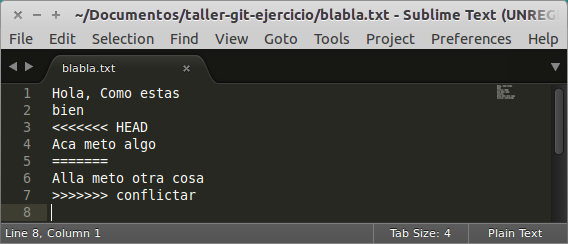
\includegraphics[height=1.0in]{images/conflicto.png}
    \end{block}

    \begin{block}{¿Qué hago?}
        \begin{itemize}
        \item Decido cómo tiene que quedar el archivo final
        \pause
        \item Hago add
		\pause
        \item
        Despues commit normalmente, con un mensaje como 'Merge'
        \end{itemize}
    \end{block}

\end{frame}


\begin{frame}[t]{Creando un repositorio vacío}
    \begin{comando}
        git init
    \end{comando}

    \pause
    \begin{block}{}
        Crea un repositorio local vacío. Un lienzo en blanco, por así decirlo.
        \begin{enumerate}
            \item Nos paramos en el directorio que queremos convertir en un repositorio.
            \item Ejecutamos \texttt{git init}.
        \end{enumerate}
        Esto crea un subdirectorio \textit{.git} que tiene todos los archivos necesarios de Git.
    \end{block}
\end{frame}

\begin{frame}[t]{Vinculando un repositorio remoto}
    \begin{comando}
        git remote
    \end{comando}

    \vspace{0.5em}
    \pause
    \begin{block}{Ver los repositorios remotos asociados}
        Ejecutamos \texttt{git remote -v}.
    \end{block}

    \pause
    \begin{block}{Agregar un repositorio remoto}
        Ejecutamos \texttt{git remote add [nombre que queramos] [URL]}.
    \end{block}
\end{frame}

\begin{frame}[t]{¡A practicar!}

    \begin{ejercicio}{Ejercicio de a 2 máquinas (preferiblemente 2 personas): 👾 y 👽}
        \begin{enumerate}\begin{small}
            \pause
            \item 👾 y 👽: crear un repositorio local vacío.
            \pause
            \item 👾: crear un repositorio nuevo en \href{https://www.gitlab.com}{GitLab},
            y darle permiso a 👽 para hacer \textit{push}.
            \pause
            \item 👾 y 👽: asociar el repositorio remoto recién creado.
            \pause
            \item 👾 y 👽: crear un archivo \textit{README} con contenidos distintos en la primera línea.
            \pause
            \item 👾: hacer \textit{push} de los cambios al repositorio remoto.
            \pause
            \item 👽: intentar hacer \textit{push} de los cambios al repositorio remoto. ¿Qué pasó?
            \pause
            \item 👽: bajarse los cambios del repositorio remoto. ¿Anduvo?
            \pause
            \item 👽: resolver los conflictos que haya.
            \pause
            \item 👽: añadir y confirmar el archivo que tenía conflicto.
            \pause
            \item 👽: \textit{pushear} estos nuevos cambios.
            \pause
            \item 👾: bajarse los nuevos cambios.
        \end{small}\end{enumerate}
    \end{ejercicio}

\end{frame}
